% !Rnw weave = knitr
\documentclass{article}\usepackage[]{graphicx}\usepackage[]{color}
% maxwidth is the original width if it is less than linewidth
% otherwise use linewidth (to make sure the graphics do not exceed the margin)
\makeatletter
\def\maxwidth{ %
  \ifdim\Gin@nat@width>\linewidth
    \linewidth
  \else
    \Gin@nat@width
  \fi
}
\makeatother

\definecolor{fgcolor}{rgb}{0.345, 0.345, 0.345}
\newcommand{\hlnum}[1]{\textcolor[rgb]{0.686,0.059,0.569}{#1}}%
\newcommand{\hlstr}[1]{\textcolor[rgb]{0.192,0.494,0.8}{#1}}%
\newcommand{\hlcom}[1]{\textcolor[rgb]{0.678,0.584,0.686}{\textit{#1}}}%
\newcommand{\hlopt}[1]{\textcolor[rgb]{0,0,0}{#1}}%
\newcommand{\hlstd}[1]{\textcolor[rgb]{0.345,0.345,0.345}{#1}}%
\newcommand{\hlkwa}[1]{\textcolor[rgb]{0.161,0.373,0.58}{\textbf{#1}}}%
\newcommand{\hlkwb}[1]{\textcolor[rgb]{0.69,0.353,0.396}{#1}}%
\newcommand{\hlkwc}[1]{\textcolor[rgb]{0.333,0.667,0.333}{#1}}%
\newcommand{\hlkwd}[1]{\textcolor[rgb]{0.737,0.353,0.396}{\textbf{#1}}}%
\let\hlipl\hlkwb

\usepackage{framed}
\makeatletter
\newenvironment{kframe}{%
 \def\at@end@of@kframe{}%
 \ifinner\ifhmode%
  \def\at@end@of@kframe{\end{minipage}}%
  \begin{minipage}{\columnwidth}%
 \fi\fi%
 \def\FrameCommand##1{\hskip\@totalleftmargin \hskip-\fboxsep
 \colorbox{shadecolor}{##1}\hskip-\fboxsep
     % There is no \\@totalrightmargin, so:
     \hskip-\linewidth \hskip-\@totalleftmargin \hskip\columnwidth}%
 \MakeFramed {\advance\hsize-\width
   \@totalleftmargin\z@ \linewidth\hsize
   \@setminipage}}%
 {\par\unskip\endMakeFramed%
 \at@end@of@kframe}
\makeatother

\definecolor{shadecolor}{rgb}{.97, .97, .97}
\definecolor{messagecolor}{rgb}{0, 0, 0}
\definecolor{warningcolor}{rgb}{1, 0, 1}
\definecolor{errorcolor}{rgb}{1, 0, 0}
\newenvironment{knitrout}{}{} % an empty environment to be redefined in TeX

\usepackage{alltt}

\title{Fantastic Yearly Report}
\author{me}
\date{\today}
\IfFileExists{upquote.sty}{\usepackage{upquote}}{}
\begin{document}
\section{Introduction}
Blah blah, we have this cool longitudinal data we want to study, let's do it! 

%% Script generates/knits all of the appropriate sections individually
\begin{knitrout}
\definecolor{shadecolor}{rgb}{0.969, 0.969, 0.969}\color{fgcolor}\begin{kframe}
\begin{alltt}
\hlkwd{source}\hlstd{(}\hlstr{'generateSections.R'}\hlstd{)}
\end{alltt}


{\ttfamily\noindent\itshape\color{messagecolor}{\#\# \\\#\# \\\#\# processing file: templateSection.Rnw}}\begin{verbatim}
## 
  |                                                                            
  |                                                                      |   0%
  |                                                                            
  |..........                                                            |  14%
##    inline R code fragments
## 
## 
  |                                                                            
  |....................                                                  |  29%
## label: unnamed-chunk-2 (with options) 
## List of 1
##  $ results: chr "hide"
## 
## 
  |                                                                            
  |..............................                                        |  43%
##   ordinary text without R code
## 
## 
  |                                                                            
  |........................................                              |  57%
## label: histogram
## 
  |                                                                            
  |..................................................                    |  71%
##   ordinary text without R code
## 
## 
  |                                                                            
  |............................................................          |  86%
## label: unnamed-chunk-3
## 
  |                                                                            
  |......................................................................| 100%
##   ordinary text without R code
\end{verbatim}


{\ttfamily\noindent\itshape\color{messagecolor}{\#\# output file: year1.tex\\\#\# \\\#\# \\\#\# \\\#\# processing file: templateSection.Rnw}}

{\ttfamily\noindent\bfseries\color{errorcolor}{\#\# Error in parse\_block(g[-1], g[1], params.src): duplicate label 'unnamed-chunk-1'}}\end{kframe}
\end{knitrout}

%% Now drop them here:
% !Rnw root = masterReport.Rnw
\section{Year 1 results}
Here is our ``data'' from year 1.
\begin{knitrout}
\definecolor{shadecolor}{rgb}{0.969, 0.969, 0.969}\color{fgcolor}\begin{kframe}
\begin{alltt}
\hlkwd{set.seed}\hlstd{(y)}
\hlstd{yearData} \hlkwb{=} \hlkwd{rnorm}\hlstd{(}\hlnum{1000}\hlstd{,} \hlkwc{mean} \hlstd{= y)}
\hlstd{knitr}\hlopt{::}\hlstd{opts_chunk}\hlopt{$}\hlkwd{set}\hlstd{(}\hlkwc{fig.path} \hlstd{=} \hlkwd{paste0}\hlstd{(}\hlstr{'year'}\hlstd{,y,}\hlstr{'/'}\hlstd{))}
\end{alltt}
\end{kframe}
\end{knitrout}
Now let's make a plot:
\begin{knitrout}
\definecolor{shadecolor}{rgb}{0.969, 0.969, 0.969}\color{fgcolor}\begin{kframe}
\begin{alltt}
\hlkwd{hist}\hlstd{(yearData)}
\end{alltt}
\end{kframe}
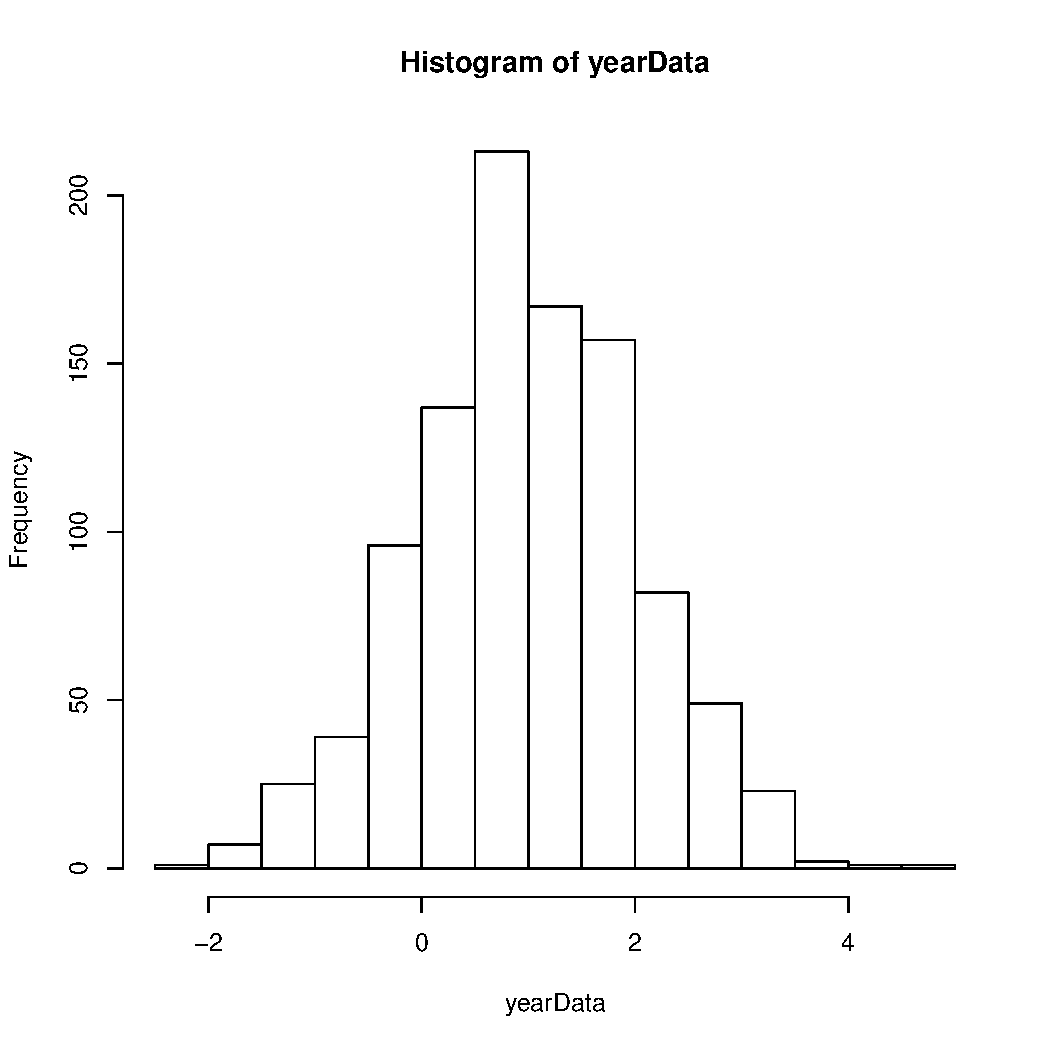
\includegraphics[width=\maxwidth]{year1/histogram-1} 

\end{knitrout}
And let's view the summary:
\begin{knitrout}
\definecolor{shadecolor}{rgb}{0.969, 0.969, 0.969}\color{fgcolor}\begin{kframe}
\begin{alltt}
\hlkwd{summary}\hlstd{(yearData)}
\end{alltt}
\begin{verbatim}
##    Min. 1st Qu.  Median    Mean 3rd Qu.    Max. 
## -2.0080  0.3026  0.9647  0.9884  1.6884  4.8103
\end{verbatim}
\end{kframe}
\end{knitrout}


% !Rnw root = masterReport.Rnw
\section{Year 2 results}
Here is our ``data'' from year 2.
\begin{knitrout}
\definecolor{shadecolor}{rgb}{0.969, 0.969, 0.969}\color{fgcolor}\begin{kframe}
\begin{alltt}
\hlkwd{set.seed}\hlstd{(y)}
\hlstd{yearData} \hlkwb{=} \hlkwd{rnorm}\hlstd{(}\hlnum{1000}\hlstd{,} \hlkwc{mean} \hlstd{= y)}
\hlstd{knitr}\hlopt{::}\hlstd{opts_chunk}\hlopt{$}\hlkwd{set}\hlstd{(}\hlkwc{fig.path} \hlstd{=} \hlkwd{paste0}\hlstd{(}\hlstr{'year'}\hlstd{,y,}\hlstr{'/'}\hlstd{))}
\end{alltt}
\end{kframe}
\end{knitrout}
Now let's make a plot:
\begin{knitrout}
\definecolor{shadecolor}{rgb}{0.969, 0.969, 0.969}\color{fgcolor}\begin{kframe}
\begin{alltt}
\hlkwd{hist}\hlstd{(yearData)}
\end{alltt}
\end{kframe}
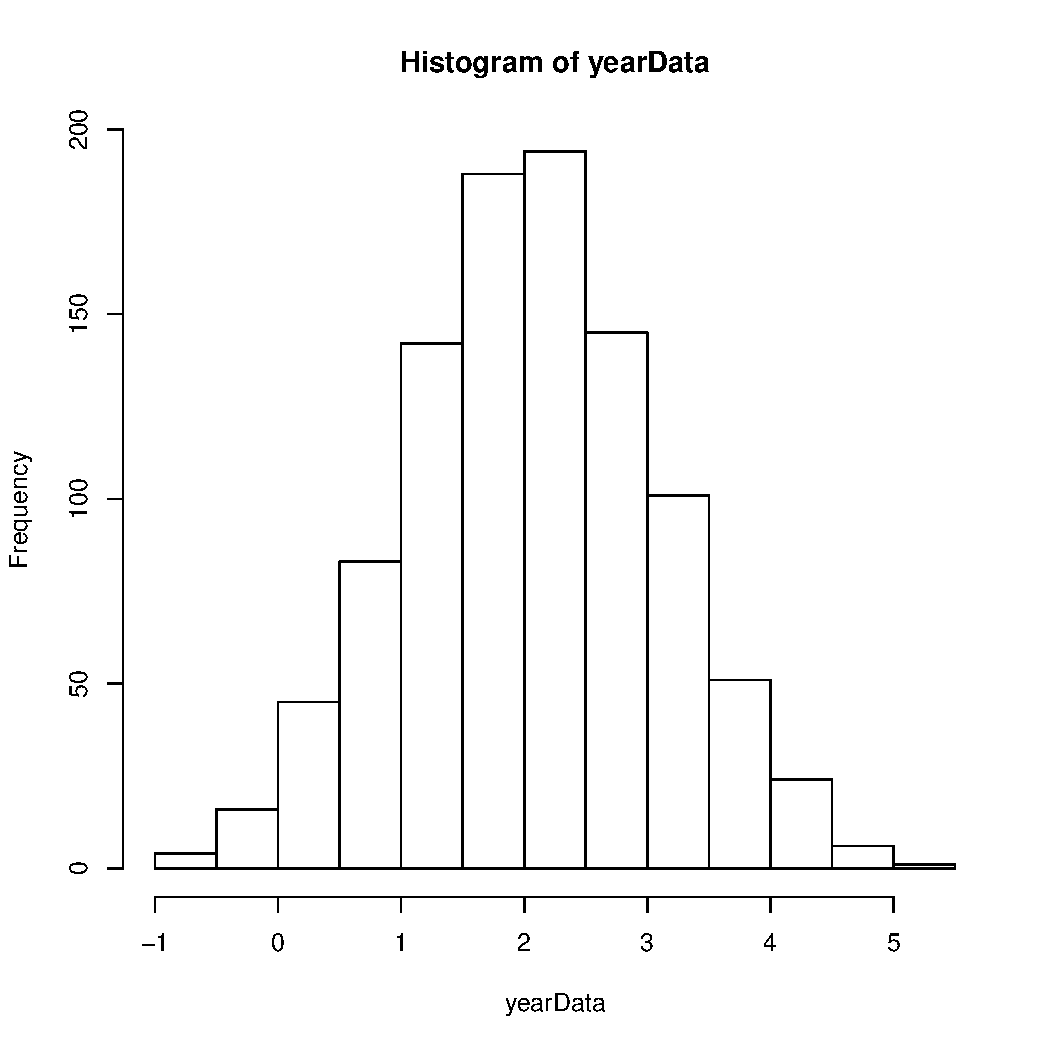
\includegraphics[width=\maxwidth]{year2/histogram-1} 

\end{knitrout}
And let's view the summary:
\begin{knitrout}
\definecolor{shadecolor}{rgb}{0.969, 0.969, 0.969}\color{fgcolor}\begin{kframe}
\begin{alltt}
\hlkwd{summary}\hlstd{(yearData)}
\end{alltt}
\begin{verbatim}
##    Min. 1st Qu.  Median    Mean 3rd Qu.    Max. 
## -0.7218  1.3687  2.0501  2.0620  2.7711  5.0088
\end{verbatim}
\end{kframe}
\end{knitrout}


% !Rnw root = masterReport.Rnw
\section{Year 3 results}
Here is our ``data'' from year 3.
\begin{knitrout}
\definecolor{shadecolor}{rgb}{0.969, 0.969, 0.969}\color{fgcolor}\begin{kframe}
\begin{alltt}
\hlkwd{set.seed}\hlstd{(y)}
\hlstd{yearData} \hlkwb{=} \hlkwd{rnorm}\hlstd{(}\hlnum{1000}\hlstd{,} \hlkwc{mean} \hlstd{= y)}
\hlstd{knitr}\hlopt{::}\hlstd{opts_chunk}\hlopt{$}\hlkwd{set}\hlstd{(}\hlkwc{fig.path} \hlstd{=} \hlkwd{paste0}\hlstd{(}\hlstr{'year'}\hlstd{,y,}\hlstr{'/'}\hlstd{))}
\end{alltt}
\end{kframe}
\end{knitrout}
Now let's make a plot:
\begin{knitrout}
\definecolor{shadecolor}{rgb}{0.969, 0.969, 0.969}\color{fgcolor}\begin{kframe}
\begin{alltt}
\hlkwd{hist}\hlstd{(yearData)}
\end{alltt}
\end{kframe}
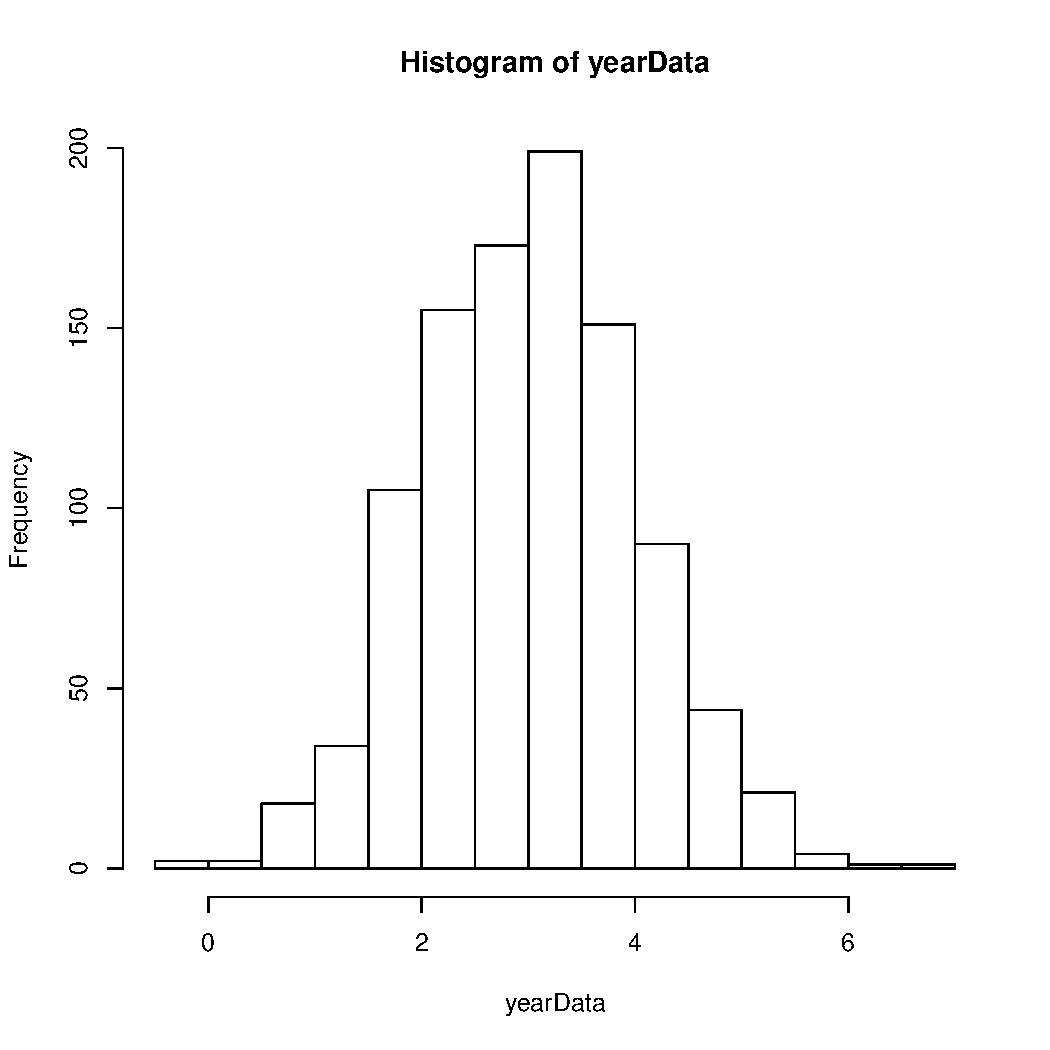
\includegraphics[width=\maxwidth]{year3/histogram-1} 

\end{knitrout}
And let's view the summary:
\begin{knitrout}
\definecolor{shadecolor}{rgb}{0.969, 0.969, 0.969}\color{fgcolor}\begin{kframe}
\begin{alltt}
\hlkwd{summary}\hlstd{(yearData)}
\end{alltt}
\begin{verbatim}
##     Min.  1st Qu.   Median     Mean  3rd Qu.     Max. 
## -0.05633  2.31546  3.03234  3.00640  3.67667  6.51930
\end{verbatim}
\end{kframe}
\end{knitrout}


% !Rnw root = masterReport.Rnw
\section{Year 4 results}
Here is our ``data'' from year 4.
\begin{knitrout}
\definecolor{shadecolor}{rgb}{0.969, 0.969, 0.969}\color{fgcolor}\begin{kframe}
\begin{alltt}
\hlkwd{set.seed}\hlstd{(y)}
\hlstd{yearData} \hlkwb{=} \hlkwd{rnorm}\hlstd{(}\hlnum{1000}\hlstd{,} \hlkwc{mean} \hlstd{= y)}
\hlstd{knitr}\hlopt{::}\hlstd{opts_chunk}\hlopt{$}\hlkwd{set}\hlstd{(}\hlkwc{fig.path} \hlstd{=} \hlkwd{paste0}\hlstd{(}\hlstr{'year'}\hlstd{,y,}\hlstr{'/'}\hlstd{))}
\end{alltt}
\end{kframe}
\end{knitrout}
Now let's make a plot:
\begin{knitrout}
\definecolor{shadecolor}{rgb}{0.969, 0.969, 0.969}\color{fgcolor}\begin{kframe}
\begin{alltt}
\hlkwd{hist}\hlstd{(yearData)}
\end{alltt}
\end{kframe}
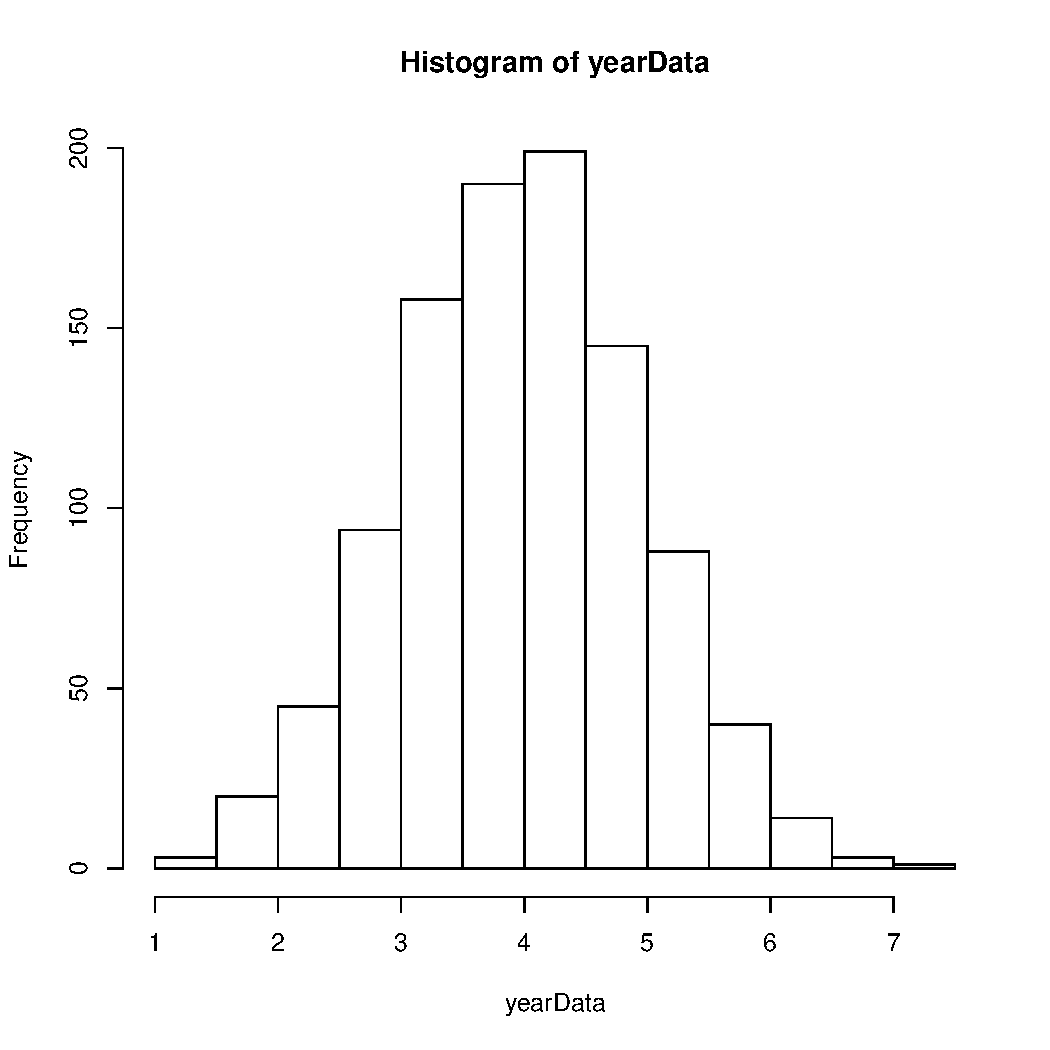
\includegraphics[width=\maxwidth]{year4/histogram-1} 

\end{knitrout}
And let's view the summary:
\begin{knitrout}
\definecolor{shadecolor}{rgb}{0.969, 0.969, 0.969}\color{fgcolor}\begin{kframe}
\begin{alltt}
\hlkwd{summary}\hlstd{(yearData)}
\end{alltt}
\begin{verbatim}
##    Min. 1st Qu.  Median    Mean 3rd Qu.    Max. 
##   1.160   3.334   3.960   3.966   4.635   7.174
\end{verbatim}
\end{kframe}
\end{knitrout}


% !Rnw root = masterReport.Rnw
\section{Year 5 results}
Here is our ``data'' from year 5.
\begin{knitrout}
\definecolor{shadecolor}{rgb}{0.969, 0.969, 0.969}\color{fgcolor}\begin{kframe}
\begin{alltt}
\hlkwd{set.seed}\hlstd{(y)}
\hlstd{yearData} \hlkwb{=} \hlkwd{rnorm}\hlstd{(}\hlnum{1000}\hlstd{,} \hlkwc{mean} \hlstd{= y)}
\hlstd{knitr}\hlopt{::}\hlstd{opts_chunk}\hlopt{$}\hlkwd{set}\hlstd{(}\hlkwc{fig.path} \hlstd{=} \hlkwd{paste0}\hlstd{(}\hlstr{'year'}\hlstd{,y,}\hlstr{'/'}\hlstd{))}
\end{alltt}
\end{kframe}
\end{knitrout}
Now let's make a plot:
\begin{knitrout}
\definecolor{shadecolor}{rgb}{0.969, 0.969, 0.969}\color{fgcolor}\begin{kframe}
\begin{alltt}
\hlkwd{hist}\hlstd{(yearData)}
\end{alltt}
\end{kframe}
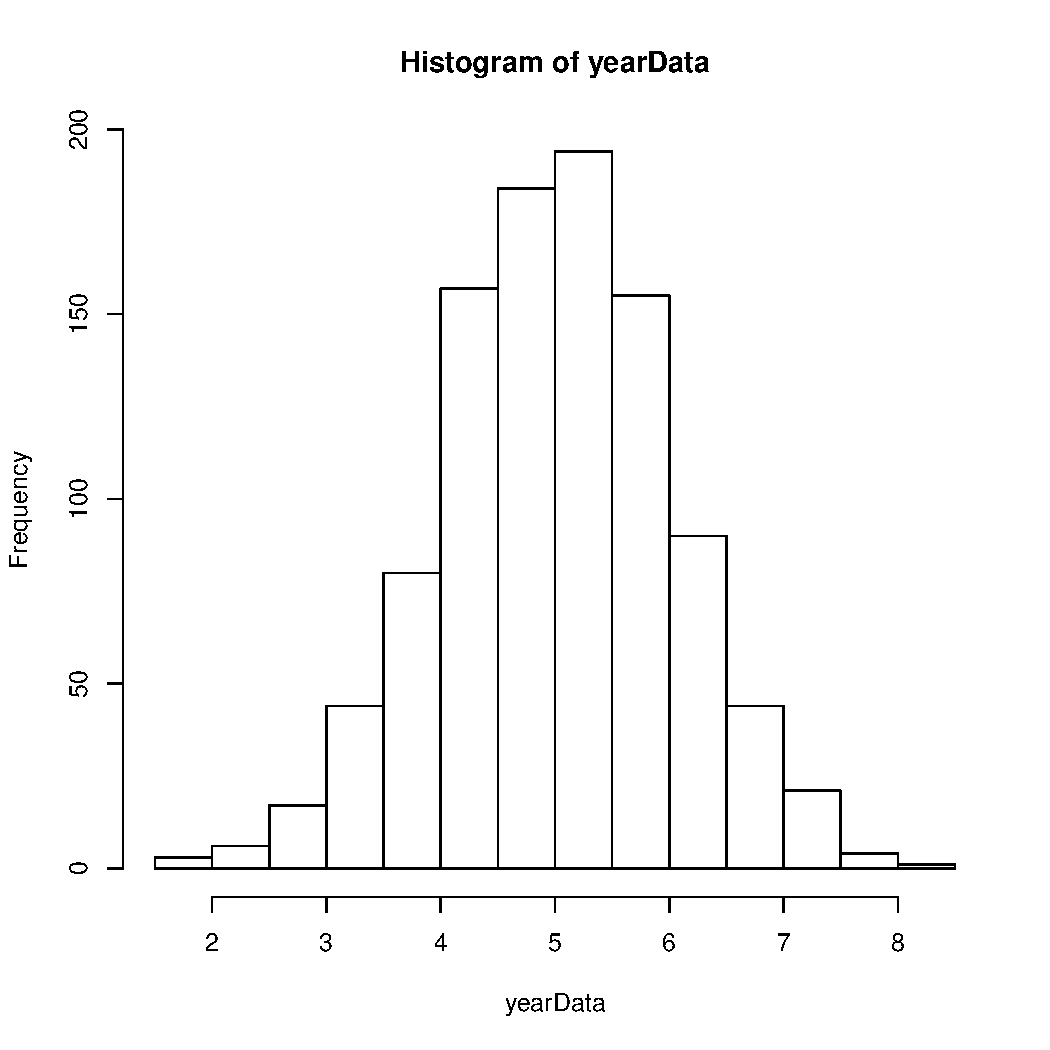
\includegraphics[width=\maxwidth]{year5/histogram-1} 

\end{knitrout}
And let's view the summary:
\begin{knitrout}
\definecolor{shadecolor}{rgb}{0.969, 0.969, 0.969}\color{fgcolor}\begin{kframe}
\begin{alltt}
\hlkwd{summary}\hlstd{(yearData)}
\end{alltt}
\begin{verbatim}
##    Min. 1st Qu.  Median    Mean 3rd Qu.    Max. 
##   1.502   4.344   5.022   5.017   5.692   8.402
\end{verbatim}
\end{kframe}
\end{knitrout}



\end{document}
